\begin{frame}{BDE drawings, parts and software are already available}
  \begin{columns}[T,onlytextwidth]
    \begin{column}{0.47\textwidth}
      \textbf{TPC protection panel designs}\par\medskip
      \colorbox{DunePaper}{\includegraphics[page=2,width=\dimexpr\linewidth-2\fboxsep\relax,height=3.1cm,keepaspectratio,
        trim=290bp 500bp 900bp 430bp,clip]{figures/tpc-panel-reference.pdf}}\par
      \medskip\DuneDiagramCaption{Central PLC, bias I/O and LV/fan/heater reference panels.}
    \end{column}
    \begin{column}{0.49\textwidth}
      \textbf{BDE Ignition screens}\par\medskip
      \includegraphics[page=7,width=\linewidth,height=3.1cm,keepaspectratio,
        trim=10bp 210bp 460bp 74bp,clip]{figures/sc-progress-june2026.pdf}\par
      \planningnote{Existing display of WIEC groups; June 2026 SC progress presentation.}
    \end{column}
  \end{columns}\par
  \medskip
  Parts list: CX5140 PLC, EK1100 couplers, EK1521 fibre links and EL2124 inhibit outputs.
  \planningnote{Historical TPC reference: EDMS 2401090 v4, sheet 2, with parts and power workbooks. The VD baseline is eight WIECs per group.}
\end{frame}

\begin{frame}{BDE cooling already has an input-to-inhibit path}
  \centering
  \begin{tikzpicture}[
    box/.style={fill=DunePaper,text=DuneOnAccent,align=center,
      text width=1.75cm,minimum height=1.25cm,inner sep=4pt,font=\small},
    edge/.style={-{Stealth},draw=DuneSky,line width=1.2pt}]
    \node[box] (fan) at (-5.75,0.6) {Fan status\\DB25 cable};
    \node[box] (input) at (-3.45,0.6) {EL1004\\input I/O};
    \node[box,fill=DuneSky] (plc) at (-1.15,0.6) {DPS PLC\\cooling rule};
    \node[box] (output) at (1.15,0.6) {EL2124\\5 V output};
    \node[box,fill=DuneCoral] (supply) at (3.45,0.6) {PL506\\channel inhibit};
    \node[box] (load) at (5.75,0.6) {Affected WIEC\\48 V feed};
    \draw[edge] (fan) -- (input);
    \draw[edge] (input) -- (plc);
    \draw[edge] (plc) -- (output);
    \draw[edge] (output) -- (supply);
    \draw[edge] (supply) -- (load);
    \node[font=\small] at (-2.3,1.55) {EtherCAT};
    \node[font=\small] at (0,1.55) {EtherCAT};
    \node[font=\small] at (2.3,1.55) {Wired};
  \end{tikzpicture}\par
  \medskip
  \DuneDiagramCaption{Cooling fault $\rightarrow$ withdraw the permit for the affected PL506 channel.}
  \medskip
  \raggedright \textbf{Feedback:} PL506 state and voltage/current $\rightarrow$ SNMP $\rightarrow$ DPS;
  OPC UA carries the result to SC for logging.\par
  \medskip
  \textbf{VD allocation check:} six fan-status signals per WIEC means 48 per
  eight-WIEC group. Match these to the populated VD inputs and cables.\par
  \planningnote{The six-fan WIEC note differs from the four-fan ICEBERG reference. These are baseline requirements, not new-module counts. Fan voting and allowed shutdown time remain to be agreed.}
\end{frame}

\begin{frame}{Backup: DAPHNE paths in the working ICD}
 \centering
 \resizebox{0.84\linewidth}{!}{% Adapted from icd-sc-pds/sections/03_protocols_services.tex at bfb2a8b.
\begin{tikzpicture}[
 box/.style={fill=DunePaper,text=DuneOnAccent,align=center,font=\small,inner sep=5pt},
 flow/.style={-{Stealth},draw=DuneSky,line width=1.2pt},
 both/.style={arrows={Stealth-Stealth},draw=DuneSky,line width=1.2pt}]
\node[box,text width=37mm] (ignition) at (0,0)
 {SC server\\OPC UA client\\$\rightarrow$ Ignition};
\node[box,text width=32mm] (daq) at (5.0,0) {DAQ CCM client\\opmon subscriber};
\node[box,text width=35mm] (hermesclient) at (10.7,0)
 {DAQ Hermes\\configuration client};
\node[box,text width=75mm,minimum height=19mm] (ua) at (2.5,-2.3)
 {SC bridge server\\ZMQ client $\rightarrow$ OPC UA bridge\\Integrated DAQ configuration};
\node[box,text width=49mm,minimum height=18mm] (daphne) at (2.5,-5.2)
 {DAPHNE\\AXI / OS $\rightarrow$ daphne-server\\$\rightarrow$ ZMQ};
\node[box,text width=37mm,minimum height=18mm] (hermes) at (10.7,-5.2)
 {Board-side Hermes\\IPBus / UDP\\Configuration endpoint};
\node[draw=DuneSky,dashed,rounded corners,fit=(daphne)(hermes),inner sep=8pt,
 label={[font=\small,text=DuneSky]below:One DAPHNE board; one shared 1\,Gb Ethernet CCM connection}] {};
\draw[both] (ignition) -- node[left,font=\small]{OPC UA} (ignition |- ua.north);
\draw[both] (daq) -- node[right,font=\small]{OPC UA} (daq |- ua.north);
\draw[both] ([xshift=-11mm]ua.south) -- node[left,align=right,font=\small,fill=DuneBackground,inner sep=2pt]
 {Configuration\\request/response} ([xshift=-11mm]daphne.north);
\draw[flow,draw=DuneSky] ([xshift=11mm]daphne.north) -- node[right,align=left,font=\small,fill=DuneBackground,inner sep=2pt]
 {Published\\monitoring} ([xshift=11mm]ua.south);
\draw[both] (hermesclient.south) -- node[right,align=left,font=\small]
 {IPBus / UDP\\configuration} (hermes.north);
\end{tikzpicture}
}\par
 \DuneDiagramCaption{Working SC--PDS--DPS ICD, Figure 1. DAQ CCM/opmon and Hermes remain distinct clients.}
\end{frame}

\begin{frame}{Backup: VD rack space and the existing DPS allocation}
  \renewcommand{\arraystretch}{1.4}
  \begin{tabularx}{\textwidth}{@{}>{\RaggedRight\arraybackslash}p{3.4cm}r>{\RaggedRight\arraybackslash}X@{}}
    \toprule
    \textbf{Rack type} & \textbf{Count} & \textbf{DPS allocation and workbook space}\\
    \midrule
    BDE auxiliary & 10 & 12U DPS; U3--U21 marked Space (19U); eight WIECs per rack\\
    BDE low voltage & 20 & One PL506 per rack; four WIECs per supply\\
    Bias high voltage & 10 & 12U DPS; U3--U12 marked Space (10U)\\
    \bottomrule
  \end{tabularx}\par
  \bigskip
  Space marked in the rack workbook is not a new DPS reservation.
  Free DIN-rail length and I/O capacity depend on the populated VD panel.
  \planningnote{May 2025 VD workbook: BDE Aux Rack and Bias HV Rack. Auxiliary U9 also has a possible ground-plane readout note. U is rack height.}
\end{frame}

\begin{frame}{The VD bias-panel draft specifies two DIN rails per rack}
  \renewcommand{\arraystretch}{1.3}
  \begin{tabularx}{\textwidth}{@{}>{\RaggedRight\arraybackslash}Xrr@{}}
    \toprule
    \textbf{Component} & \textbf{Per rail} & \textbf{10 racks}\\
    \midrule
    EK1100 EtherCAT coupler & 1 & 20\\
    EL9410 supply terminal & 1 & 20\\
    EL2124: four 5 V outputs & 18 & 360\\
    EL9011 end cap & 1 & 20\\
    24 V power supply & 1 & 20\\
    \bottomrule
  \end{tabularx}\par
  \medskip
  Each rail occupies 337 mm. The draft provides 1,440 output channels;
  the working VD inventory lists 576 bias channels.\par
  \planningnote{May 2025 workbook, Bias HV Rack!K17:K21. This is the first-pass layout; the difference from 576 bias channels is not verified spare capacity.}
\end{frame}

\begin{frame}{Use the component loads for the VD power budget}
  \small
  \renewcommand{\arraystretch}{1.3}
  \begin{tabularx}{\textwidth}{@{}>{\RaggedRight\arraybackslash}p{3.7cm}>{\RaggedRight\arraybackslash}p{2.4cm}>{\RaggedRight\arraybackslash}X@{}}
    \toprule
    \textbf{Equipment} & \textbf{Power / capacity} & \textbf{Basis and limit}\\
    \midrule
    PL506 input & 2.25 kW each & 20 supplies: about 45.1 kW expected AC input\\
    WIEC fans only & 380 W per group & $8\times6\times0.33\,\mathrm{A}\times24\,\mathrm{V}$; excludes heaters and I/O\\
    Bias DPS supply allowance & 24 V, 40 A & 960 W DC capacity per rack in the workbook\\
    \bottomrule
  \end{tabularx}\par
  \medskip
  The inherited 831 W auxiliary figure needs a VD component budget
  covering fans, heaters and populated I/O.\par
  \planningnote{May workbook; WIEC safety note, internal revision 0. Fan arithmetic assumes six fans per WIEC. Rated load, expected AC input and DC supply capacity are distinct.}
\end{frame}

\begin{frame}{Rack infrastructure already has a hardware reference}
  \small
  \renewcommand{\arraystretch}{1.2}
  \begin{tabularx}{\textwidth}{@{}>{\RaggedRight\arraybackslash}p{3.4cm}>{\RaggedRight\arraybackslash}X@{}}
    \toprule
    \textbf{Rack component} & \textbf{Reference hardware / allocation}\\
    \midrule
    PDU & Raritan PX3; inlet and outlet allocation for the connected loads\\
    Smoke detector & 4WTAR-B and EOLR-1 end-of-line relay\\
    Contact interface & DX-PD2C5; 12 V supply to the smoke detector\\
    Humidity & Record the probe and peripheral interface for each rack\\
    Temperature / water leak & PDU peripheral sensors where fitted\\
    \bottomrule
  \end{tabularx}\par
  \medskip
  \normalsize The May workbook includes a 76-entry rack-protection/PDU allowance.
  Map the actual rack packages against this existing allowance.\par
  \planningnote{DUNE-doc-32655 v8, sections 3 and 5; May workbook, Standard Rack and Power Summary!B28. The guide does not specify a humidity probe model or trip requirement.}
\end{frame}

\begin{frame}{Reference: local PDU trips and recovery}
  \renewcommand{\arraystretch}{1.45}
  \begin{tabularx}{\textwidth}{@{}>{\RaggedRight\arraybackslash}p{3.7cm}>{\RaggedRight\arraybackslash}X@{}}
    \toprule
    \textbf{PX3 setup guide} & \textbf{Local behaviour documented}\\
    \midrule
    Smoke, water, temperature & Local event rules and scripts can switch off the protected outlets\\
    Network-switch outlet & Kept powered during the guide's fallback shutdown\\
    After a local trip & Power is restored deliberately; no automatic restoration\\
    \bottomrule
  \end{tabularx}\par
  \bigskip
  The VD control chain is Ignition $\rightarrow$ DPS PLC $\rightarrow$ PDU.
  Local trip status returns to the PLC and to SC for logging.
  \planningnote{DUNE-doc-32655 v8 describes an Ignition-direct prototype with local fallback on loss of Ignition. The VD PLC command path requires matching reachability, trip and reset configuration; it is not a claim that the prototype already implements it.}
\end{frame}

\begin{frame}{The VD inventory covers the other subsystem connections}
  \renewcommand{\arraystretch}{1.35}
  \begin{tabularx}{\textwidth}{@{}>{\RaggedRight\arraybackslash}p{3.2cm}>{\RaggedRight\arraybackslash}X@{}}
    \toprule
    \textbf{Subsystem} & \textbf{Working inventory and interfaces}\\
    \midrule
    PDS readout / calibration & 34 LV feeds in the current presentation scope; supply status and control interfaces\\
    Power over fibre (PoF) & 80 boxes; 320 voltage and 80 temperature readings; Opta PLC or Beckhoff PLC alternative\\
    TDE & 20 mezzanine racks; PDU control now; other TDE interfaces are possible extensions\\
    Calibration / cryogenic instrumentation & Level and temperature readout, purity monitors, ionization laser and neutron source\\
    \bottomrule
  \end{tabularx}
  \planningnote{Subsystem exchanges use OPC UA through SC. PoF uses the current 4 V + 1 temperature case; these readings do not count central DPS terminals.}
\end{frame}

\begin{frame}{The BMS drawing identifies 20 control-panel symbols}
  \renewcommand{\arraystretch}{1.4}
  \begin{tabularx}{\textwidth}{@{}>{\RaggedRight\arraybackslash}p{3.4cm}>{\RaggedRight\arraybackslash}X@{}}
    \toprule
    \textbf{Drawing area} & \textbf{Interfaces on the inspection maps}\\
    \midrule
    CUC, level 4850 & Eight panel references: air handling, chilled water, power and associated equipment\\
    Level 4910 & North and south sump interfaces, SP-1 and SP-2\\
    4850-08-ES group & Spare panel for future equipment; mapped to the access-drift inspection area\\
    Other 4850 areas & Chillers, pumps, ventilation and generator interfaces\\
    \bottomrule
  \end{tabularx}\par
  \medskip
  Inspection planned with Rachel; Dale Curran is the SDSTA integration contact identified for this work.
  \planningnote{U-FD-M-901 rev12, 14 February 2025; marked 4850/4910 maps and survey register. Symbols are drawing references; field observations are pending.}
\end{frame}

\begin{frame}{Reference: the May 2025 VD rack inventory}
  \renewcommand{\arraystretch}{1.15}
  \begin{tabularx}{\textwidth}{@{}>{\RaggedRight\arraybackslash}Xr>{\RaggedRight\arraybackslash}Xr@{}}
    \toprule
    \textbf{Rack type} & \textbf{Count} & \textbf{Rack type} & \textbf{Count}\\
    \midrule
    BDE low voltage & 20 & PDS low voltage & 4\\
    BDE auxiliary & 10 & Drift HV & 2\\
    TDE & 20 & Reserved drift HV & 2\\
    Bias HV & 10 & Spare / CalCI & 8\\
    \bottomrule
  \end{tabularx}\par
  \bigskip
  \textbf{76 numbered mezzanine positions:} SEDM-01 to SEDM-76.\par
  \medskip
  The worksheet also has a separate concept for 40 top-plate mini-racks.
  \planningnote{May 2025 allocation: rack positions, distinct from PLC panels and remote-I/O stations. Includes the listed reserved and spare positions.}
\end{frame}
